\documentclass[10pt]{article}
\usepackage[usenames]{color} %used for font color
\usepackage{amssymb} %maths
\usepackage{amsmath} %maths
\usepackage{bbold} % indicators
\usepackage[utf8]{inputenc} %useful to type directly diacritic characters
\usepackage{tikz}
\begin{document}
\[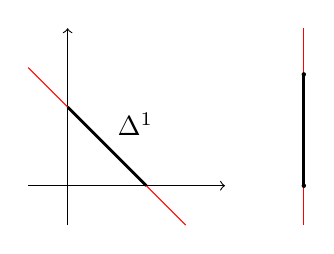
\begin{tikzpicture}
  \draw[->] (0, -1/2) -- (0, 2);
  \draw[->] (-1/2, 0) -- (2, 0);

  \draw[color = red] (3/2, -1/2) -- (-1/2, 3/2);
  
  \draw[line width = 1pt] (1,0) -- node[above right] {\(\Delta^1\)} (0,1);

  \draw[color = red] (3, -1/2) -- (3, 2);

  \draw[line width = 1pt] (3, 0) -- (3, 1.414);

  \node[circle, fill = black, inner sep = 0.2mm] at (3, 0) {};
  \node[circle, fill = black, inner sep = 0.2mm] at (3, 1.414) {};
\end{tikzpicture}\]
\end{document}